
\chapter{Analyse des outils connus}
\label{outils_connus}

\section{Java}

La version 8 de Java, qui a introduit les \TT{Stream}s, a chang\'e compl\`etement la façon dont les d\'eveloppeurs peuvent traiter les donn\'ees. La manipulation des \TT{Stream}s ressemble \`a un langage de requ\^ete de base de donn\'ees. Au lieu de parcourir les donn\'ees, les d\'eveloppeurs fournissent simplement des op\'erations \`a effectuer sur le flux. \cite{urma2014java} fournissent une description d\'etaill\'ee des nouveaux concepts introduits dans \TT{Java~8}. Les  \TT{Stream}s et \TT{Lambda}-expressions sont les fonctionnalit\'es les plus remarquables ajout\'ees dans l'API \citep{javaStreamAPI}. Ils sont con\c{c}us pour traiter les sources de donn\'ees de mani\`ere simple et efficace. Cette section d\'ecrit quelques-uns des concepts de \TT{Java~8}.


\subsection{Lambda-expressions}

Une expression lambda --- souvent appel\'ee fonction anonyme --- est un bloc de code avec des param\`etres qui peut \^etre transmis afin de pouvoir \^etre ex\'ecut\'e ult\'erieurement. Par exemple, l'expression lambda suivante re\c{c}oit deux valeurs de type entier en argument et renvoie leur somme~:
{\small
\begin{lstlisting}
 (int x, int y) -> { x + y }
\end{lstlisting}
} 


\GT{Remarque concernant les citations~: il y a deux macros que tu peux
utiliser: cite vs.\ citep: tu dois utiliser cite si tu veux que les
noms d'auteurs apparaissent comme sujet dans une phrase (avec
l'ann\'ee entre parenth\`eses)~; tu dois utiliser citep si tu veux que
la r\'ef\'erence soit compl\`etement entre parenth\`eses. Voir les
exemples ci-haut et ci-bas.}


Les expressions lambda rendent le code plus concis et \'etendent \TT{Java} avec des concepts de langages de programmation fonctionnelle. Ce concept n'est pas nouveau. Il est utilis\'e dans les langages de programmation fonctionnelle tels que \TT{Haskell}~\citep{hutton2016programming} et \TT{Lisp}~\citep{steele1990common}. En Java, ce concept est li\'e \`a l'interface fonctionnelle. Un lambda peut \^etre sp\'ecifi\'e \`a la place d'une valeur dont le type est une interface fonctionnelle. Par exemple, le listage~\ref{lambdaAsFonctionalInterface} montre un exemple o\`u un \TT{thread} d\'eclar\'e en utilisant la syntaxe de classe anonyme peut \^etre \'ecrit plus facilement avec une expression lambda.

\begin{Listing}[tbp]
\begin{lstlisting}[language=java]
	Thread th = new Thread( new Runnable() {
		public void run() {
          ...
		}
	});

	Thread th = new Thread( () -> {
         ...
	});
\end{lstlisting}
\caption{Remplacement d'une classe anonyme avec une expression lambda.}
\label{lambdaAsFonctionalInterface}
\end{Listing}

Dans une expression \TT{lambda}, lors de la compilation, les types des arguments peuvent \^etre automatiquement d\'etermin\'es par le compilateur. Cette fonctionnalit\'e permet de passer des m\'ethodes comme arguments plut\^ot que de construire un objet d'une classe sp\'ecifi\'ee. Ceci permet \`a un programmeur de construire facilement des pipelines d'op\'erations fonctionnelles.


\subsection{It\'erations}

Une it\'eration est le processus de traverser une s\'equence d'\'el\'ements. Avec les \TT{stream Java}, une it\'eration peut \^etre ex\'ecut\'ee de deux mani\`eres : en tant qu'it\'eration externe ou interne. Une it\'eration est dite \emph{externe} lorsque le d\'eveloppeur contr\^ole la travers\'ee des \'el\'ements.  L'acc\`es et l'op\'eration sur chaque \'el\'ement de la collection sont d\'efinis par l'utilisateur. Par contre, une it\'eration est dite \emph{interne} lorsque la s\'equence contr\^ole elle-m\^eme tous les d\'etails du processus d'it\'eration. L'utilisateur fournit uniquement les op\'erations permettant de traiter les \'el\'ements, sans se soucier de la mani\`ere dont les \'el\'ements sont acc\'ed\'es et fournis.
L'approche interne est attrayante pour les opportunit\'es qu'elle offre aux compilateurs, notamment l'optimisation de l'exécution et les m\'ecanismes de nettoyage n\'ecessaires en arri\`ere-plan. Un autre avantage des it\'erations internes est l'efficacit\'e~: le traitement de donn\'ees peut \^etre plus efficace car il peut \^etre r\'eparti en parall\`ele parmi les cœurs de la machine.


\subsection{Flux}


Un flux est d\'efini comme une s\'equence immuable d'\'el\'ements fournissant une vari\'et\'e d'op\'erateurs et de m\'ethodes permettant de traiter une collection de donn\'ees. Le flux prend en charge les op\'erations d'agr\'egation \citep{javaStreamAggregate} s\'equentielles et parall\`eles sans se soucier de la mani\`ere dont les \'el\'ements sont stock\'es ou accessibles. Pour effectuer un traitement, les op\'erations de flux sont compos\'ees dans un \TT{pipeline}. Un \TT{pipeline} est compos\'e d'une source, z\'ero ou plusieurs op\'erations interm\'ediaires et une op\'eration terminale. Une source en peut \^etre constitu\'ee d'une collection ou de tout objet impl\'ementant l'interface qui d\'efinit le m\'ecanisme permettant d'extraire les donn\'ees de la source. 
Les op\'erations sur les flux adoptent un m\'ecanisme d'\'evaluation paresseuse. L'\'evaluation paresseuse est une m\'ethode d'optimisation du traitement qui retarde l'\'etape du calcul jusqu'\`a ce qu'il soit n\'eécessaire. En \TT{Java}, le traitement sur les \'el\'ements du flux est r\'ealis\'e seulement \`a l'initialisation de l'op\'eration finale et les \'el\'ements source ne sont consomm\'es qu'au besoin. Cela permet au compilateur d'optimiser le traitement des donn\'ees dans le \TT{pipeline}.
Une autre technique d'optimisation utilis\'ee par \TT{Java} est l'\'evaluation court-circuit\'ee (\TT{short-circuiting} en anglais). Dans un flux sont consum\'es seulement les \'el\'ements n\'ecessaires. Par exemple, dans le listage~\ref{findFirst}, l'opérateur \TT{findFirst} retourne le premier employ\'e trouv\'e dans une liste d'employ\'ee~; les \'el\'ements restants du flux sont ignor\'es.

\begin{Listing}[tbp]
\begin{lstlisting}[language=java]
	List<Employee> employees;
	Optional<Employee> employee = employees.findFirst();
\end{lstlisting}
\caption{Optimisation du traitement d'un flux en utilisant la technique de court-circuit.}
\label{findFirst}
\end{Listing}

L'un des principaux avantages des flux est qu'ils peuvent \^etre soit \'evalu\'es de fa\c{c}on s\'equentielle, soit en parall\`ele. L'\'evaluation s\'equentielle est r\'ealis\'ee en ex\'ecutant toutes les op\'erations en \TT{pipeline} sur chaque \'el\'ement du flux. Lorsqu'un flux est \'evalu\'e en parall\`ele, il utilise un type sp\'ecial d'it\'erateur appel\'e \TT{Spliterator}. Ce dernier partitionne le flux de mani\`ere r\'ecursive en se divisant lui-m\^eme pour cr\'eer des flux enfants. Ce m\'ecanisme permet aux \emph{threads} de traverser plusieurs flux en parall\`ele. Les \emph{threads} sont g\'er\'es par un groupe de \emph{threads} de type \TT{fork-join}.


\subsection{Fork-join}

Introduit en \TT{Java~7}, le \emph{framework} \TT{fork-join} permet aux d\'eveloppeurs de sp\'ecifier des t\^aches pouvant \^etre subdivis\'ees et ex\'ecut\'ees en parall\`ele sur des machines multicœurs. Il est bas\'e sur deux op\'erations : \TT{fork} et \TT{join}. L'op\'eration \TT{fork} a le r\^ole de diviser r\'ecursivement la t\^ache en plus petites sous-t\^aches ind\'ependantes jusqu'\`a ce qu'elles soient assez simples pour \^etre ex\'ecut\'ees de mani\`ere asynchrone. L'op\'eration \TT{join} a le r\^ole de fusionner les r\'esultats de toutes les sous-t\^aches de mani\`ere r\'ecursive en un seul r\'esultat.
Les sous-t\^aches obtenues par l'op\'eration \TT{fork} sont soumises \`a un \emph{pool} \TT{fork-join}. Ce dernier est composé d'un ensemble de travailleurs. Le nombre de travailleurs dans un \emph{pool} \TT{fork-join} est g\'en\'eralement limit\'e par le nombre de cœurs de la machine. Chaque travailleur peut ex\'ecuter une t\^ache \`a la fois. Les t\^aches en attente d'ex\'ecution sont stock\'ees dans une file d'attente appartenant \`a un travailleur. Une t\^ache en cours d'ex\'ecution peut g\'en\'erer de nouvelles t\^aches, qui sont ensuite mises en file d'attente pour une ex\'ecution ult\'erieure. Lorsqu'un travailleur a termin\'e l'ex\'ecution d'une t\^ache, il essaie de prendre une t\^ache des files d'attente des autres travailleurs \`a l'aide d'un algorithme de vol de travail (\emph{work stealing algorithm} en anglais). Cet algorithme permet un \'equilibrage efficace de la charge de travail entre les divers travailleurs.


\subsection{Word Count en Java}

Afin d'illustrer le mod\`ele de programmation avec les \TT{Stream}s de \TT{Java~8}, le listage~\ref{wordCountJava} montre le code source d'une application de d\'ecompte des mots --- plus pr\'ecis\'ement, l'application compte le nombre d'occurrences des divers mots dans un fichier texte. Une telle application est compos\'ee de plusieurs op\'erations encha\^in\'ees :


\begin{itemize}
	\item La premi\`ere op\'eration, \TT{Files.lines}, renvoie un flux s\'equentiel de lignes \`a partir du fichier. Le fichier est rep\'er\'e par le param\`etre \TT{inputFile} fourni en argument.

	\item La deuxi\`eme op\'eration, \TT{parallel}, marque le flux en tant que flux parall\`ele. Cette op\'eration permet ainsi de partitionner et d'ex\'ecuter le \TT{pipeline} en parall\`ele.

	\item L'op\'eration \TT{flatMap} divise chaque ligne en mots qui sont ensuite transmis en aval sous forme d'\'el\'ements de donn\'ees individuels.
	
	\item L'op\'eration \TT{map} transforme les lettres majuscules du mot en lettres minuscules.
	
	\item L'op\'eration \TT{filter} s\'electionne dans le flux seulement les mots qui ne sont pas vides.
	
	\item La deuxi\`eme op\'eration \TT{map} dans le pipeline cr\'ee un \TT{Entry} avec la cl\'e repr\'esent\'ee par le mot.
	
	\item L'op\'eration \TT{collect} collecte les \'el\'ements dans un \TT{Map} et compte la fr\'equence de mots.
	
	\item L'op\'eration \TT{entrySet} renvoie un flux de type cl\'e--valeur. La cl\'e est le mot et la valeur est sa fr\'equence dans le fichier.
	
	\item La derni\`ere op\'eration \TT{collect} collecte les \'el\'ements dans une liste.
	
	
\end{itemize}





\begin{Listing}[tbp]
\begin{lstlisting}[language=java]
  List<Map.Entry<String,Integer>> wordsCount = 
	Files.lines(Paths.get(inputFile))
    .parallel()
    .flatMap(line->Arrays.stream(line.trim().split(" ")))
    .map(word->word.replaceAll("[^a-zA-Z]", "").toLowerCase())
    .filter(word->word.length() > 0)
    .map(word->new SimpleEntry<>(word, 1))
    .collect(toMap(e->e.getKey(),e->e.getValue(),(v1,v2)->v1+v2))
    .entrySet().stream()
    .collect(Collectors.toList());
\end{lstlisting}
\caption{Le code source Java~8 d'une application de d\'ecompte du nombre d'occurrences des mots.}
\label{wordCountJava}
\end{Listing}




\section{FastFlow}

\TT{FastFlow} est une biblioth\`eque \TT{C++} qui offre un ensemble de m\'ecanismes de bas niveau pour supporter les flux de donn\'ees, et s'ex\'ecutant sur des machines multicœurs avec m\'emoire partag\'ee. La facilit\'e de d\'eveloppement et l'efficacit\'e d'ex\'ecution de \TT{FastFlow} peuvent \^etre obtenues en augmentant le niveau d'abstraction de la phase de conception. Son efficacit\'e provient principalement de la mise en œuvre optimis\'ee de m\'ecanismes de communication de bas niveau et de sa conception en couches. Il fournit aux d\'eveloppeurs un ensemble de squelettes algorithmiques qui peuvent \^etre utilis\'es pour parall\'eliser les plus courants mod\`eles de parall\'elisme. Ces squelettes algorithmiques peuvent \^etre librement imbriqu\'es pour cr\'eer des mod\`eles de parall\'elisme plus complexes.

\TT{FastFlow} a \'et\'e conçue selon plusieurs principes: conception en couches, efficacit\'e et pour supporter le parall\'elisme de flux.

\textbf{Conception en couches}

\TT{FastFlow} a \'et\'e conçue dans une pile de couches pour permettre d'impl\'ementer les m\'ecanismes d'optimisations. La figure~\ref{FastFlowLayers.fig} montre les trois principales couches: \TT{High-level patterns}, \TT{Core patterns} et \TT{Building blocks}. 

Le niveau le plus bas de la pile, \TT{Building blocks}, g\`ere les communications asynchrones entre les canaux et g\`ere le cycle de vie des flux. Plus pr\'ecis\'ement, cette couche offre des services pour les couches sup\'erieures. Elle g\`ere les queues, les processeurs et les fils d'ex\'ecutions.

Au-dessus de la couche \TT{Building blocks} se trouve la couche \TT{Core patterns}, qui fournit des squelettes (gabarits) pour mod\'eliser le parall\'elisme de flux. Les trois mod\`eles fournis dans cette couche sont \TT{task-farm}, \TT{pipeline} et \TT{feedback}, qui permettent de construire des flux parall\`eles. 

Au sommet de la pile se trouve la couche \TT{High-level patterns}, responsable d'exprimer le parall\'elisme du code s\'equentiel. Elle fournit plusieurs m\'ethodes qui couvrent les paradigmes de programmation parall\`eles les plus courants : flux de donn\'ees, parall\'elisme de donn\'ees, et  parall\'elisme de t\^aches. 

\begin{figure}[ht]
\centering
     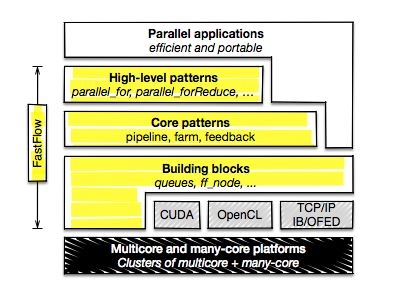
\includegraphics[width=1.0\textwidth]{Figures/FastFlowLayers.jpg}
      \caption{Les couches de FastFlow.}
       \label{FastFlowLayers.fig}
\end{figure}

\textbf{Efficacit\'e}

L'id\'ee de \TT{FastFlow} est de fournir au programmeur des files d'attente \TT{MP (Multiple Producer)} et des files d'attente \TT{MC (Multiple Consumer)} sans verrouillage afin de supporter des rapides flux de donn\'ees. G\'en\'eralement, dans les applications de flux de donn\'ees, les canaux de communication sont impl\'ementés via des files d'attente de type \TT{Multiple Producer Multiple Consumer (MPMC)}. Dans ce modèle, les files d'attente se synchronisent simultanément pour acc\'eder aux donn\'ees. Ces synchronisations sont habituellement support\'ees par une ou plusieurs op\'erations atomiques (par exemple, \TT{Compare-And-Swap}) qui se comportent comme des barri\`eres de m\'emoire. Afin d'\'eviter les barri\`eres de m\'emoires, \TT{FastFlow} b\^atit les files d'attente \TT{MPMC} en assemblant des files, sans barri\`ere de m\'emoire, de type \TT{Single Producer Single Consumer (SPSC)}. Dans ce mod\`ele, des files d’ex\'ecution regroupent ou \'emettent les donn\'ees des files d'entr\'ee vers les files de sortie. Selon son r\^ole, une file d'ex\'ecution peut \^etre un Emitter ou un Collector. Tandis que l'\TT{Emitter} lit les donn\'ees, le \TT{Collector} \'ecrit sur une ou plusieurs files d'attente de types \TT{SPSC}. Contrairement aux op\'erations atomiques, ce m\'ecanisme n\'ecessite seulement des copies de m\'emoire. La performance offerte par cette solution d\'ecoule de la vitesse sup\'erieure de la copie par rapport \`a la barri\`ere de m\'emoire.


\textbf{Parall\'elisme de flux}

Dans \TT{FastFlow} le parall\'elisme de flux est repr\'esent\'e par un flux de donn\'ees \`a l'aide d'une s\'erie d'\'etapes s\'equentielles ou parall\`eles appel\'ees stages. Chaque stage lit les donn\'ees \`a partir du flux d'entr\'ee, applique des calculs et \'ecrit le r\'esultat sur le flux de sortie. Le calcul repr\'esente une s\'equence de transformations sur les flux de donn\'ees. Le parall\'elisme est obtenu en ex\'ecutant chaque stage simultan\'ement sur d'\'el\'ements ind\'ependants ou sur sous s\'equences d'\'el\'ements. Dans FastFlow le parall\'elisme peut \^etre obtenu en exploitant directement les mod\`eles parall\`eles disponibles dans la couche \TT{Building blocks}. En particulier cela peut \^etre r\'ealis\'e:

\begin{itemize}
\item en d\'efinissant d'activit\'es concurrentes s\'equentielles en sous-classant la classe \TT{ff\_node}, et
\item en construisant des mod\`eles parall\`eles complexes en composant de mani\`ere hi\'erarchique des activit\'es concurrentes s\'equentielles, des \TT{pipelines} et des \TT{farm}.
\end{itemize}

\textbf{ff\_node}

Dans \TT{FastFlow ff\_node} est la classe de base pour le traitement du flux. Elle fournit des moyens appropri\'es pour d\'efinir d'activit\'es s\'equentielles pour le traitement de données apparaissant sur un seul canal d'entr\'ee et fournissant les r\'esultats correspondants sur un seul canal de sortie. 

La classe \TT{ff\_node} d\'efinit plusieurs m\'ethodes. Les plus importantes sont :
- virtual void*  svc (void *task) = 0
- virtual int svc\_init () { return 0 ; } 
- virtual void svc\_end ( ) {} 

La premi\`ere m\'ethode est celle qui d\'efinit le comportement du nœud lors du traitement des \'el\'ements du flux d'entr\'ee. Les deux autres m\'ethodes sont automatiquement appel\'ees lorsque le traitement repr\'esent\'e par le nœud est d\'emarr\'e \TT{(svc\_init)} et juste avant qu'elle soit termin\'ee \TT{(svc\_end)}. Ces m\'ethodes virtuelles peuvent \^etre r\'ecrites dans les sous-classes \TT{ff\_node} fournies par l'utilisateur afin d'impl\'ementer l'initialisation et la finalisation du code.


\textbf{Pipeline}

Le \TT{pipeline} est utilis\'e pour mod\'eliser les traitements exprim\'es par stages. Dans \TT{FastFlow} le \TT{pipeline} est repr\'esent\'e par la classe \TT{ff\_pipeline}. Un \TT{pipeline} peut comporter plus de deux stages et peut \^etre construit comme un pipeline \`a n stages ou comme un \TT{pipeline} de \TT{pipelines}. Un stage peut \^etre de type \TT{ff\_node} ou \TT{farm}.


\textbf{Farm}

Le \TT{farm} est le flux parall\`ele bas\'e sur la r\'eplication d'une fonction. Dans \TT{FastFlow} le \TT{farm} est repr\'esent\'e par la classe \TT{ff\_farm}. Comme le montre la figure~\ref{FastFlowFarm.fig} un \TT{farm} est compos\'e de trois parties distinctes: l'\TT{Emitter}, le \TT{pool de workers} et le \TT{Collector}. L'\TT{Emitter} est responsable de la r\'epartition des \'el\'ements de flux au \TT{pool de workers} qui traitent et produisent les donn\'ees de sortie. Les r\'esultats sont ensuite rassembl\'es par le \TT{Collector} dans un seul flux. Les communications entre \TT{Emitter} et \TT{Collector} se font via des canaux de communication sans barri\`eres de m\'emoire.

\begin{figure}[ht]
\centering
     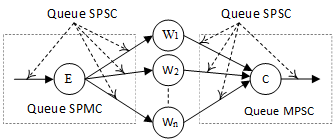
\includegraphics[width=1.0\textwidth]{Figures/FastFlowFarm.png}
      \caption{Le \TT{farm} de \TT{FastFlow} compos\'e des trois parties l'\TT{Emitter (E)}, le \TT{pool de workers (W1..Wn)} et le \TT{Collector (C)}. Les canaux de communication sont impl\'ement\'es en assemblant des files d'attente de types \TT{Simple Producer Simple Consumer (SPSC)}}.
       \label{FastFlowFarm.fig}
\end{figure}